\section{Elektronrör}
\label{elektronrör}
\index{elektronrör}

\subsection{Allmänt}

Ett elektronrör består av två eller flera elektroder i en lufttom glaskolv.

\subsection{Vakuumdioden (tvåelektrodröret)}
\textbf{HAREC a.\ref{HAREC.a.2.8.1}\label{myHAREC.a.2.8.1}}
\label{vakuumdioden}
\index{vakuumdioden}
\index{elektronrör!diod}

\begin{wrapfigure}[9]{R}{0.5\textwidth}
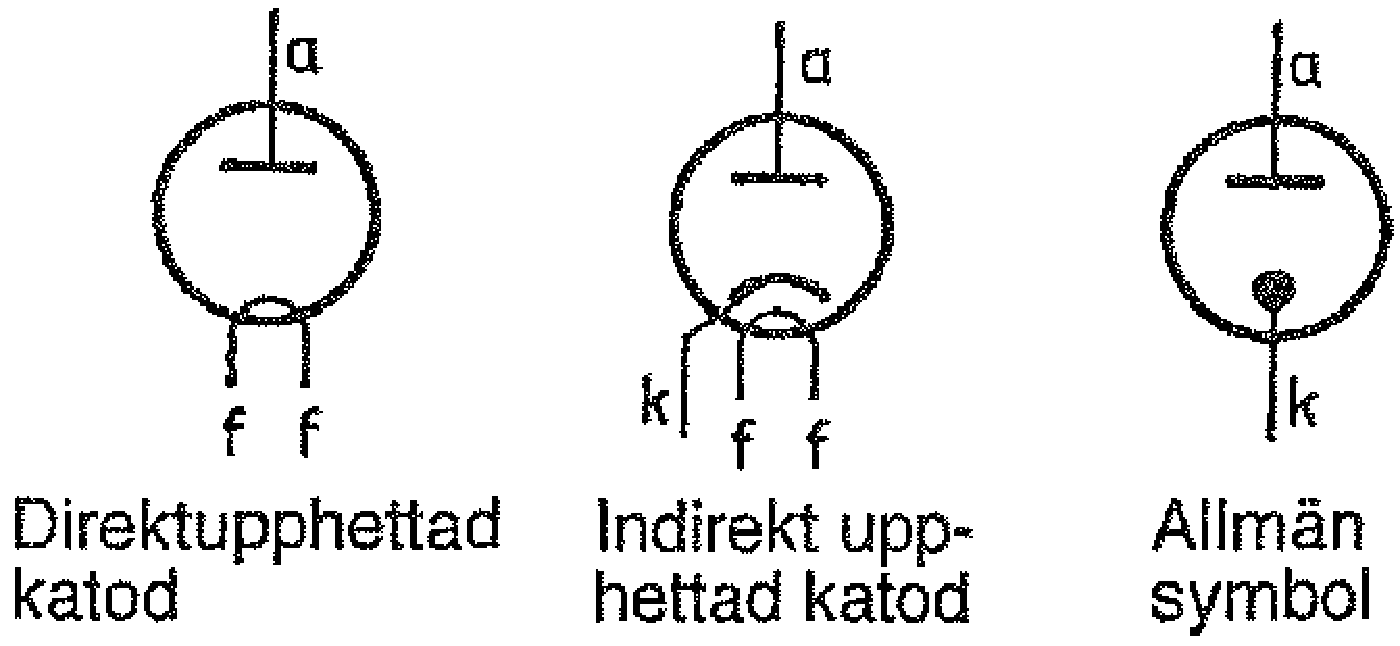
\includegraphics[width=0.5\textwidth]{images/cropped_pdfs/bild_2_2-24.pdf}
\caption{Schemasymboler för dioder}
\label{fig:BildII2-24}
\end{wrapfigure}

Bild \ref{fig:BildII2-24}

Dioden innehåller två elektroder
\begin{itemize}
\item a anod
\item k katod, med f f = glödtråd (filament)
\end{itemize}

\emph{Anoden} ska dra elektronerna från katoden.
\emph{Katoden} ska avge elektronerna och måste därför hettas upp.

Upphettningen av katoden görs på något av följande sätt:
\begin{itemize}
\item Direkt upphettning, d.v.s. katoden är i sig själv en glödtråd. En 4-
  till 6-volts strömkälla är vanligt.
\item Indirekt upphettning, d.v.s. en glödtråd omsluter och hettar upp ett
  speciellt katodmaterial. En 1,5 till 12,6~volts glödströmkälla är vanligt.
\end{itemize}

\subsubsection{Edisoneffekten}
\index{Edisoneffekten}
\index{elektronrör!Edisoneffekten}

\begin{wrapfigure}[12]{R}{0.5\textwidth}
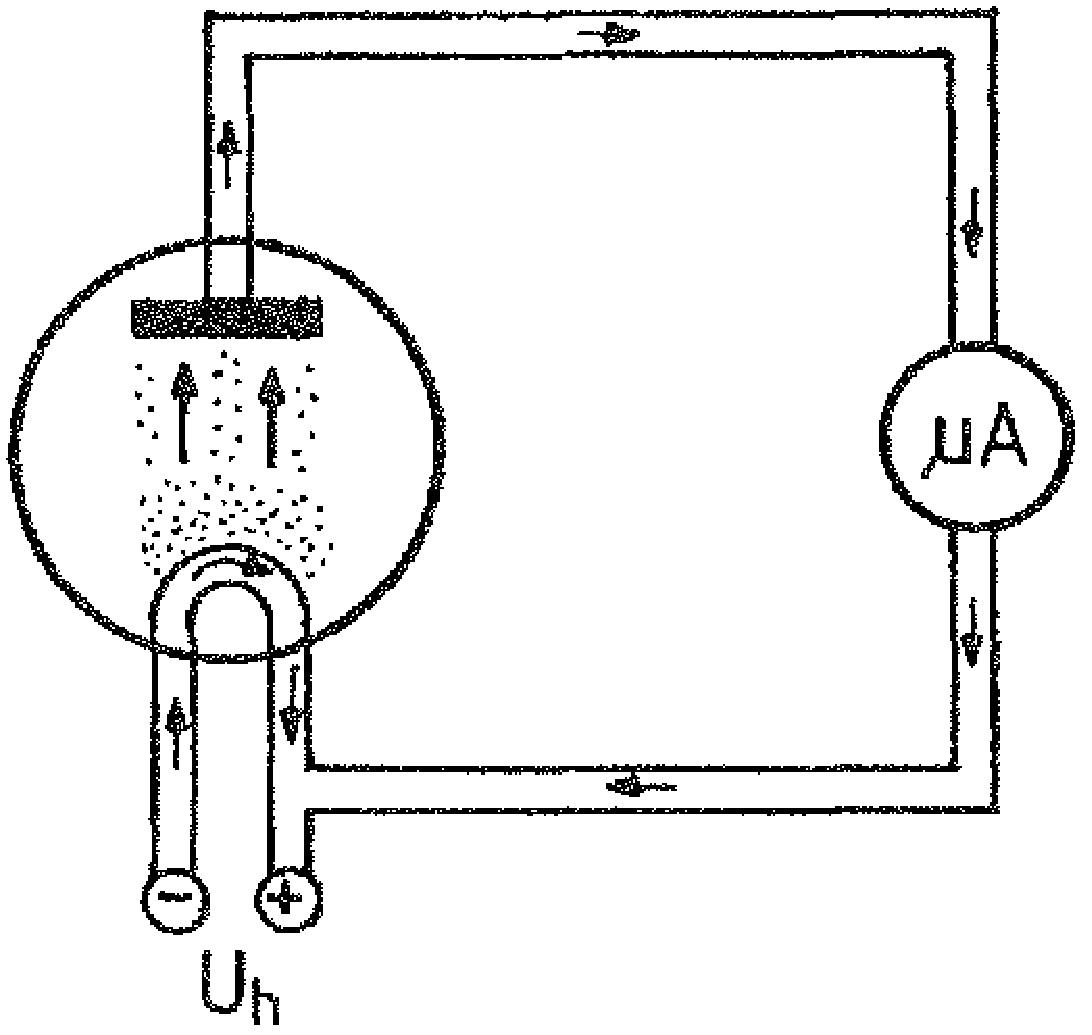
\includegraphics[width=0.5\textwidth]{images/cropped_pdfs/bild_2_2-25.pdf}
\caption{Edisoneffekten}
\label{fig:BildII2-25}
\end{wrapfigure}

Bild \ref{fig:BildII2-25}

När katoden upphettas lossnar fria elektroner från den och bildar ett moln. Med
en spänning mellan anod och katod, med anoden positiv, så kommer elektronerna
att dras mot anoden. En s.k. anodström börjar att flyta.

\subsubsection{\(I_a/U_a\)-karaktäristikan för en vakuumdiod}

\begin{figure}
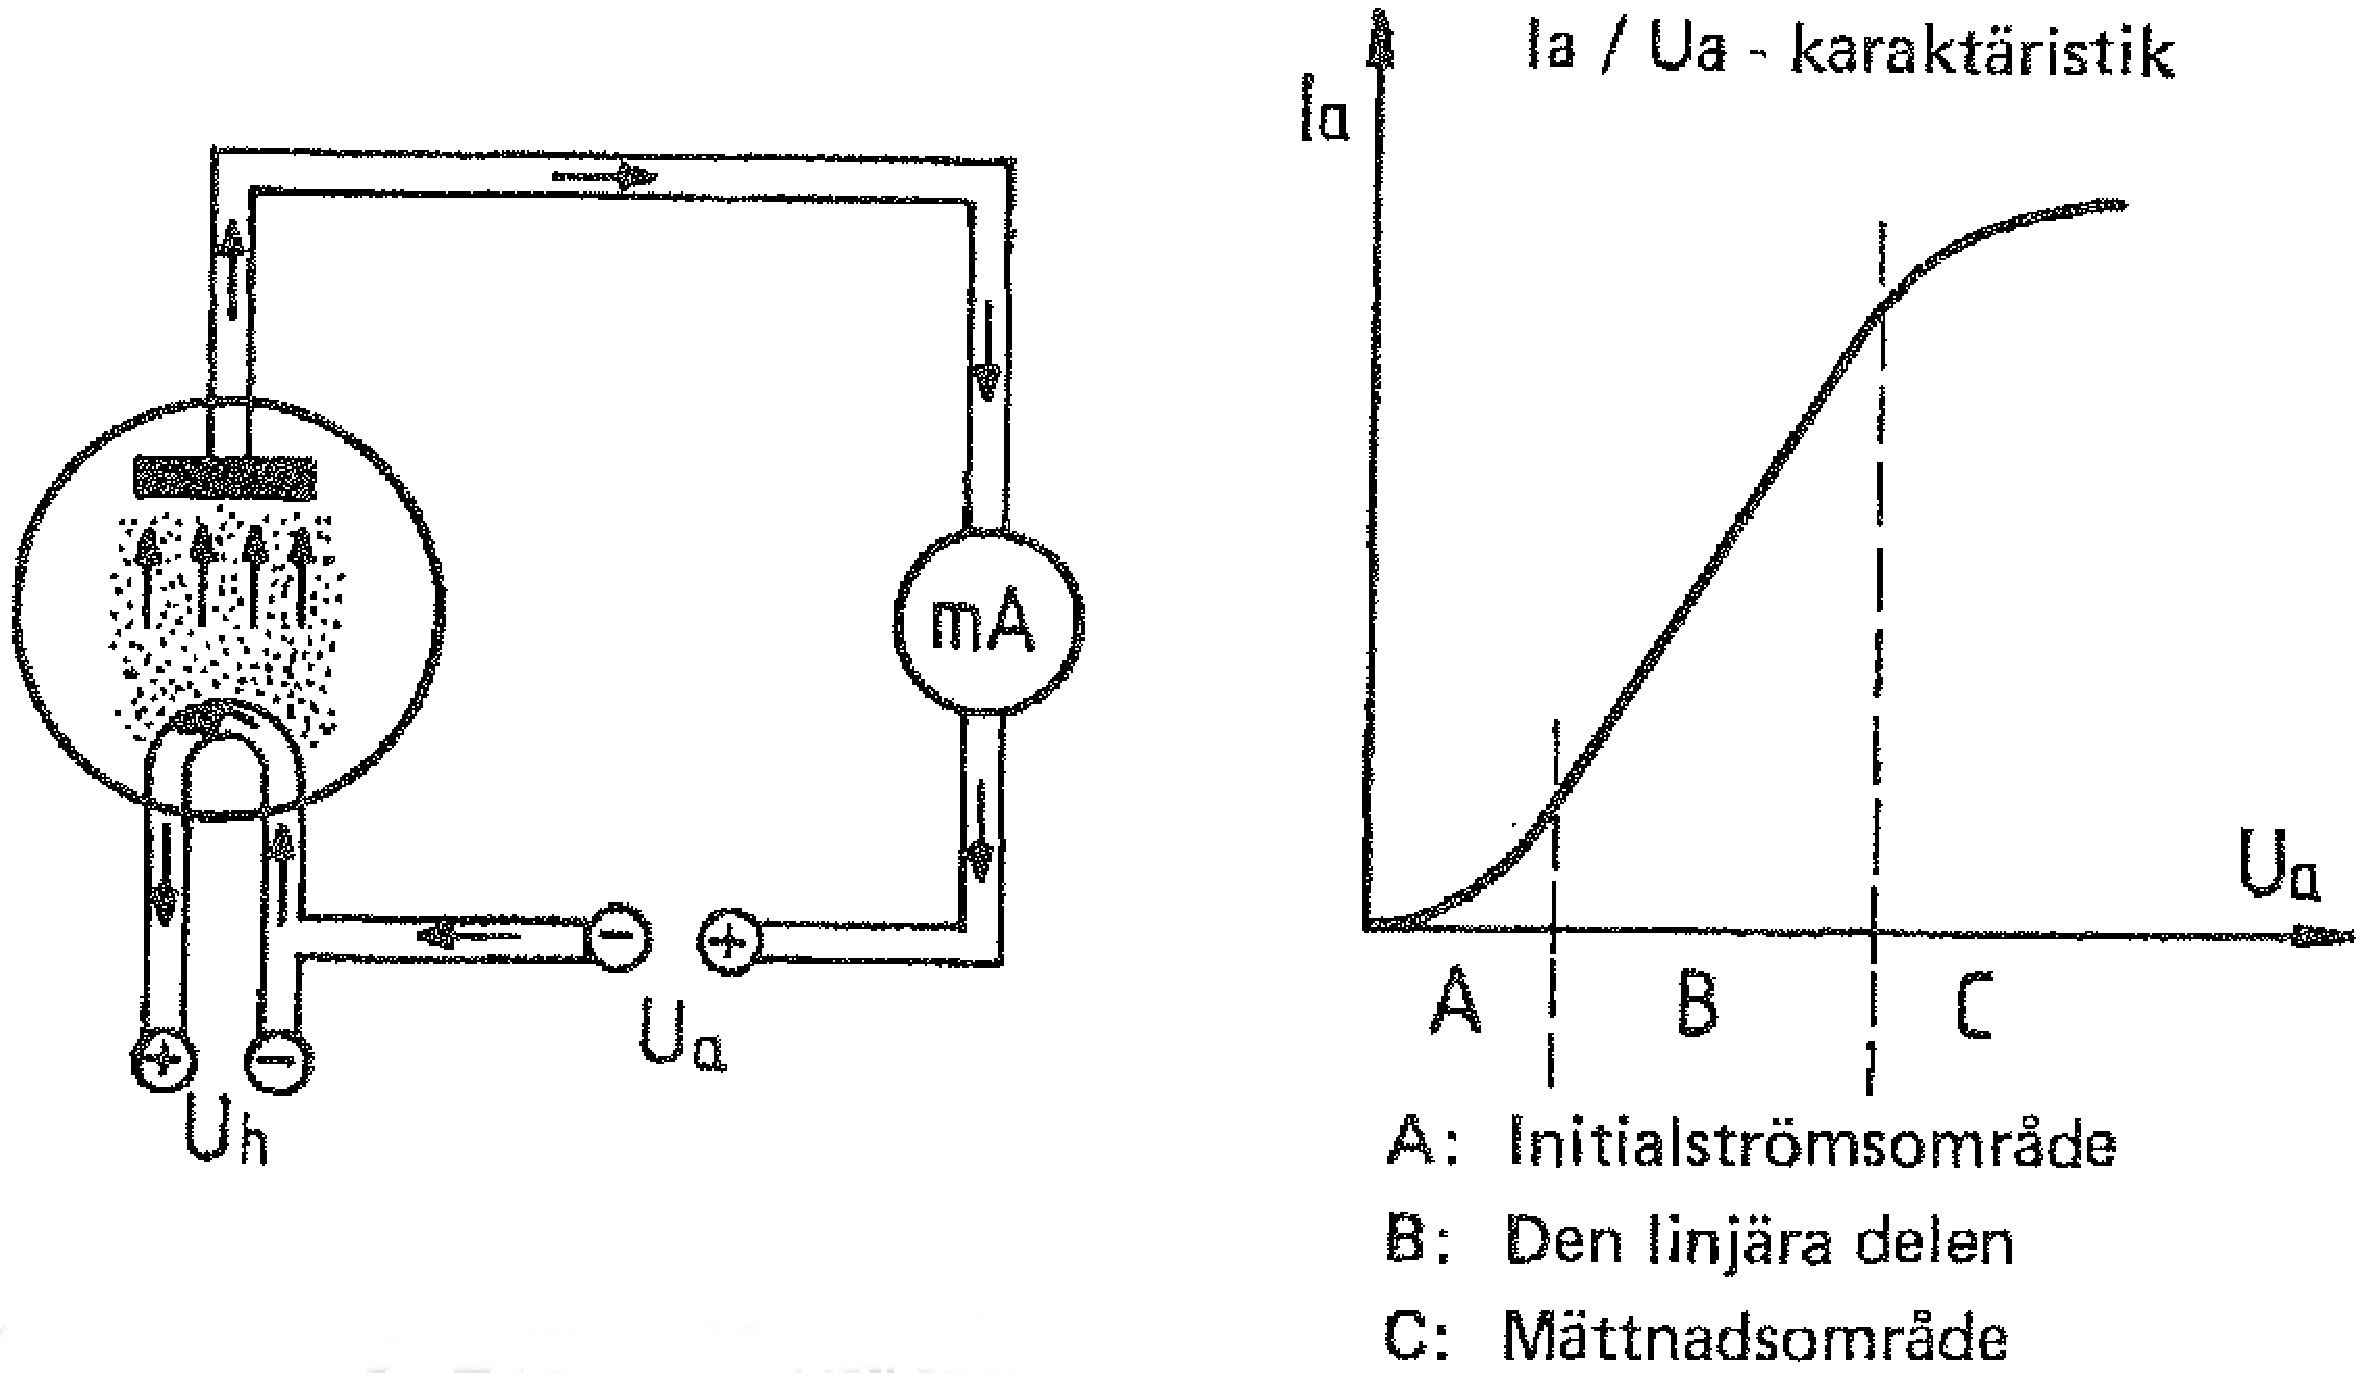
\includegraphics[width=\textwidth]{images/cropped_pdfs/bild_2_2-26.pdf}
\caption{Diodens karaktäristik}
\label{fig:BildII2-26}
\end{figure}

Bild \ref{fig:BildII2-26}

När anoden ges positiv potential (anodspänning), flyter en elektronström från
katod till anod (anodström). Om anodspänningen \(U_a\) ökar så ökar anodströmmen
\(I_a\). Varje par av talvärden representerar en punkt i ett diagram, som det på
bilden. När anodspänningen ökat till ett visst värde, så ökar inte anodströmmen
ytterligare. I ett mellanområde är kurvan
i det närmaste rak.

\subsubsection{Likriktarverkan}
\index{elektronrör!likriktarverkan}

När anoden i en vakuumdiod ges positiv potential i förhållande till katoden,
flyter en s.k. anodström förutsatt att katoden upphettas så att den avger fria
elektroner.

När anoden ges en negativ potential i förhållande till katoden flyter däremot
ingen anodström.

Vakuumdioden kan därför användas för likriktning av växelströmmar. Den har en
likriktande funktion.

\emph{Halvvågslikriktning.}

\begin{figure}
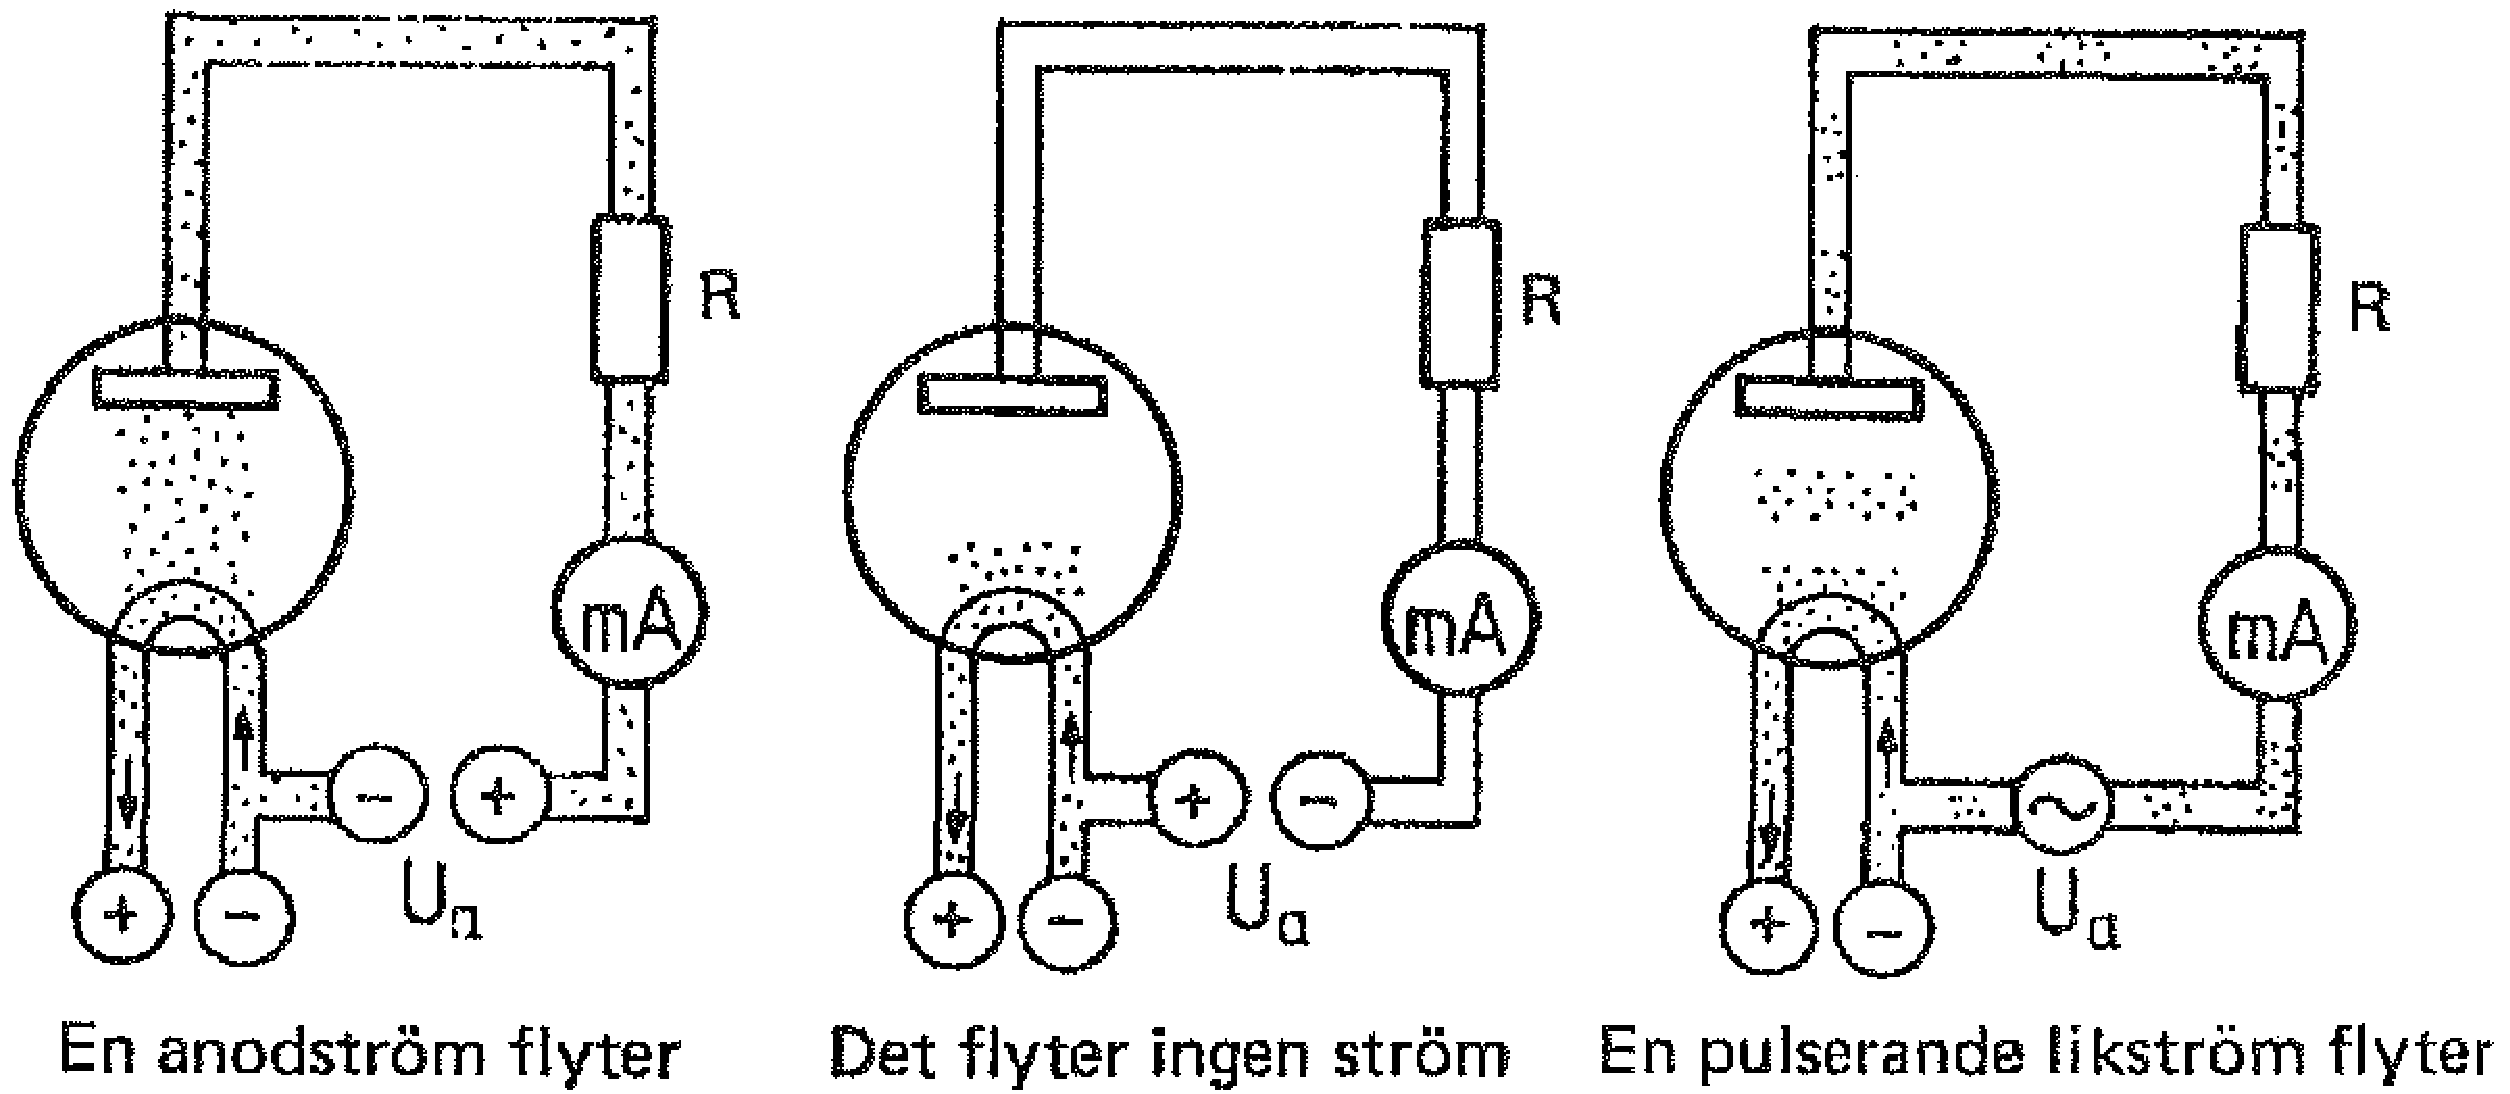
\includegraphics[width=\textwidth]{images/cropped_pdfs/bild_2_2-27.pdf}
\caption{Halvvågslikriktning}
\label{fig:BildII2-27}
\end{figure}

Bild \ref{fig:BildII2-27}

När anoden ges en omväxlande positiv och negativ potential, en växelspänning, så
flyter anodström under varje positiv halvperiod av växelspänningen. En
likströmspuls uppstår under varannan halvperiod.

\emph{Helvågslikriktning.}

\begin{figure}
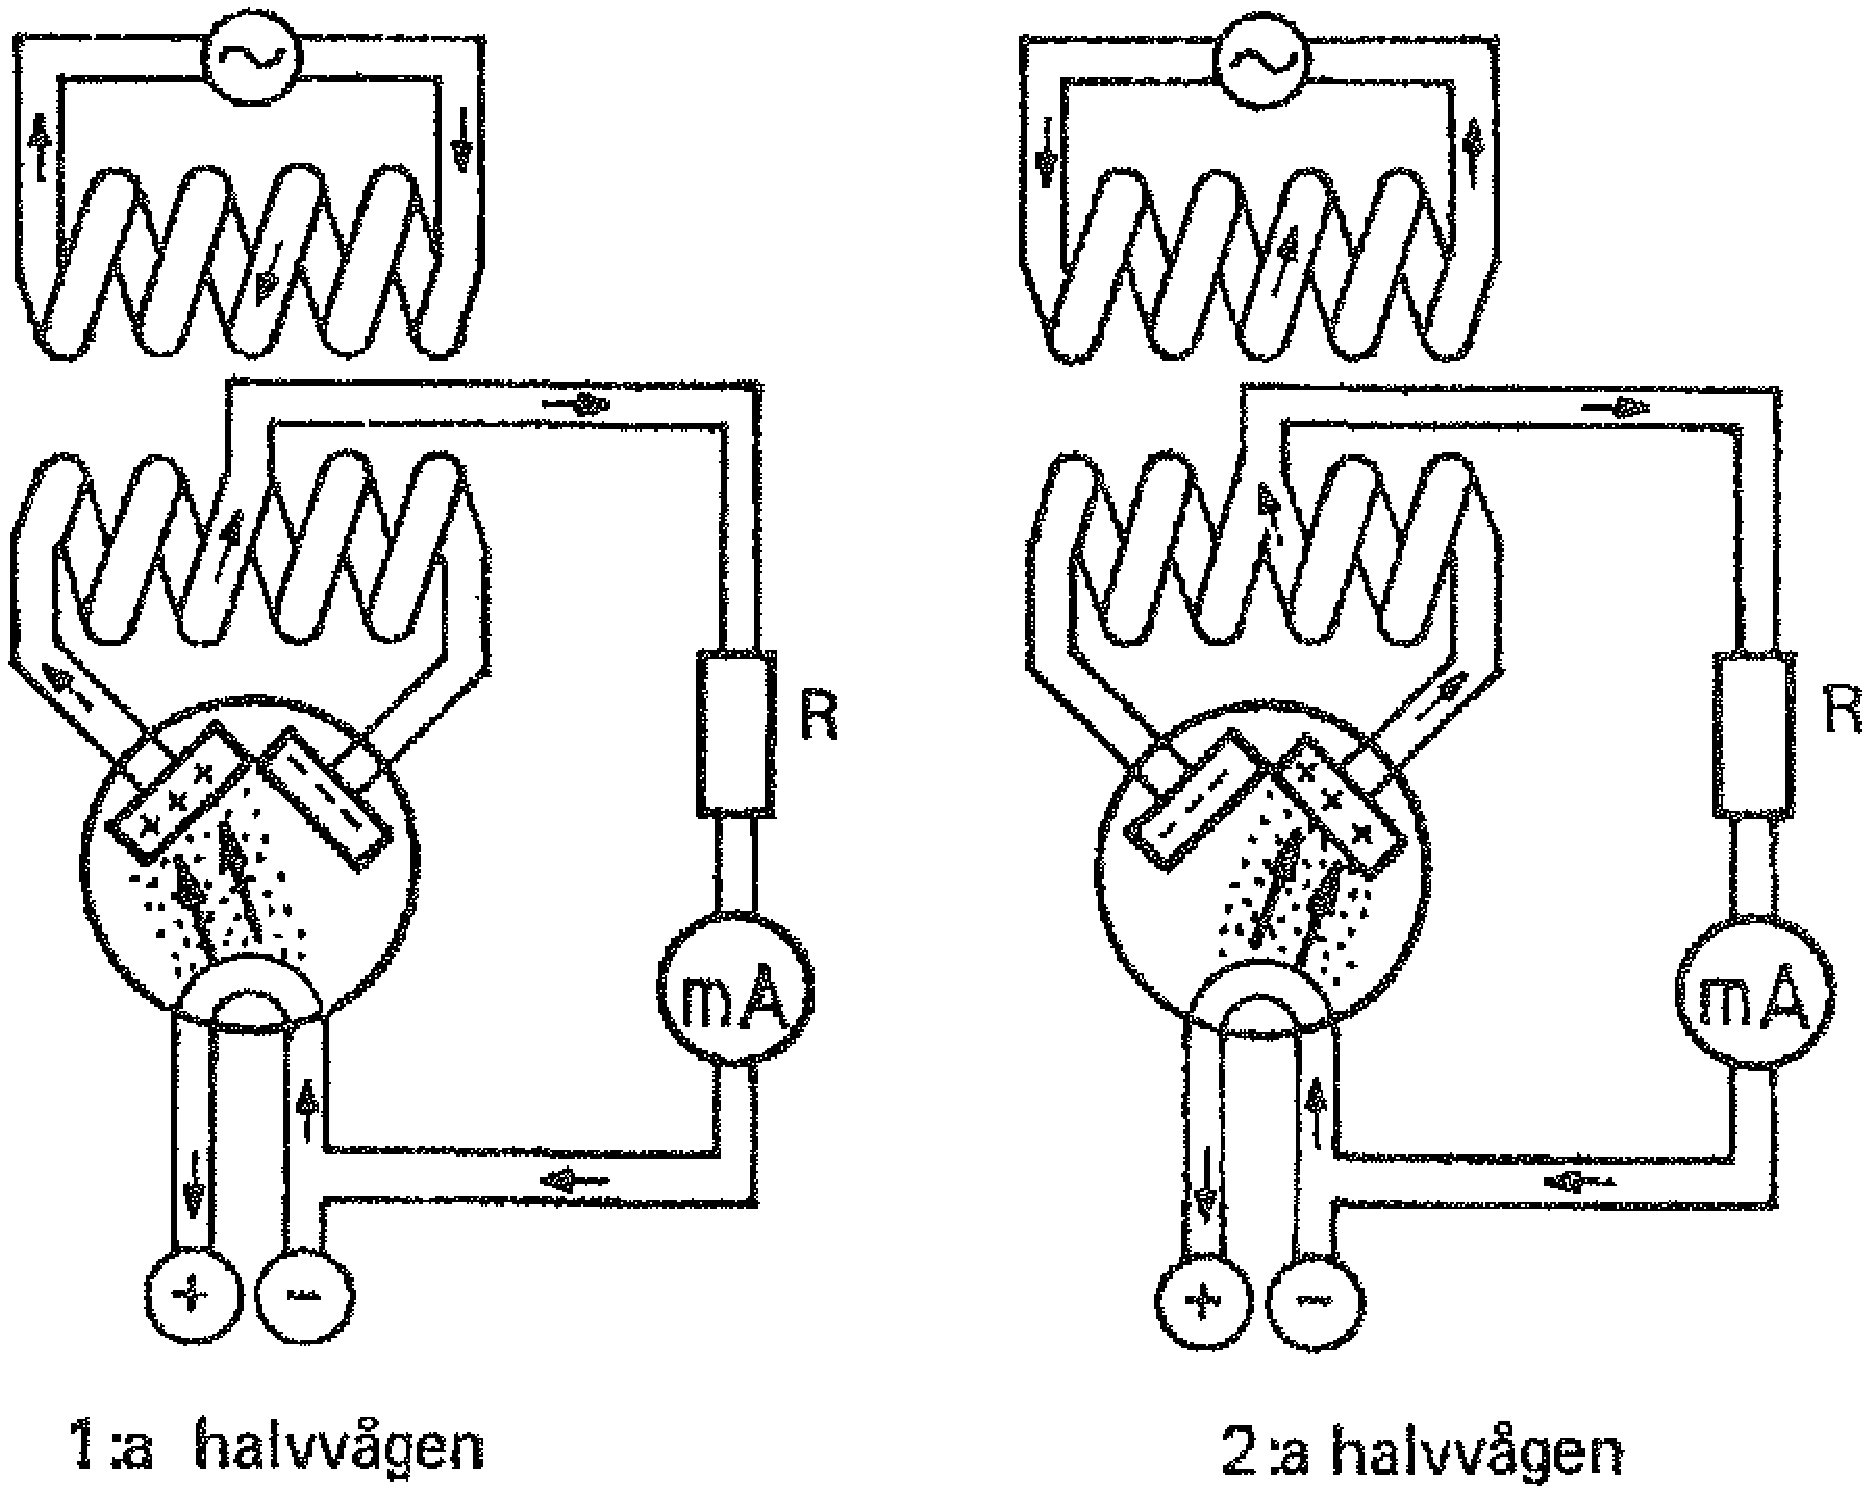
\includegraphics[width=\textwidth]{images/cropped_pdfs/bild_2_2-28.pdf}
\caption{Helvågslikriktning}
\label{fig:BildII2-28}
\end{figure}

Bild \ref{fig:BildII2-28}

Med ett elektronrör med dubbla anoder och en transformator med mittuttag på
sekundärlindningen, kan växelspänningens båda halvperioder utnyttjas så, att
anodström flyter i samma riktning under alla halvperioder.

\begin{figure}
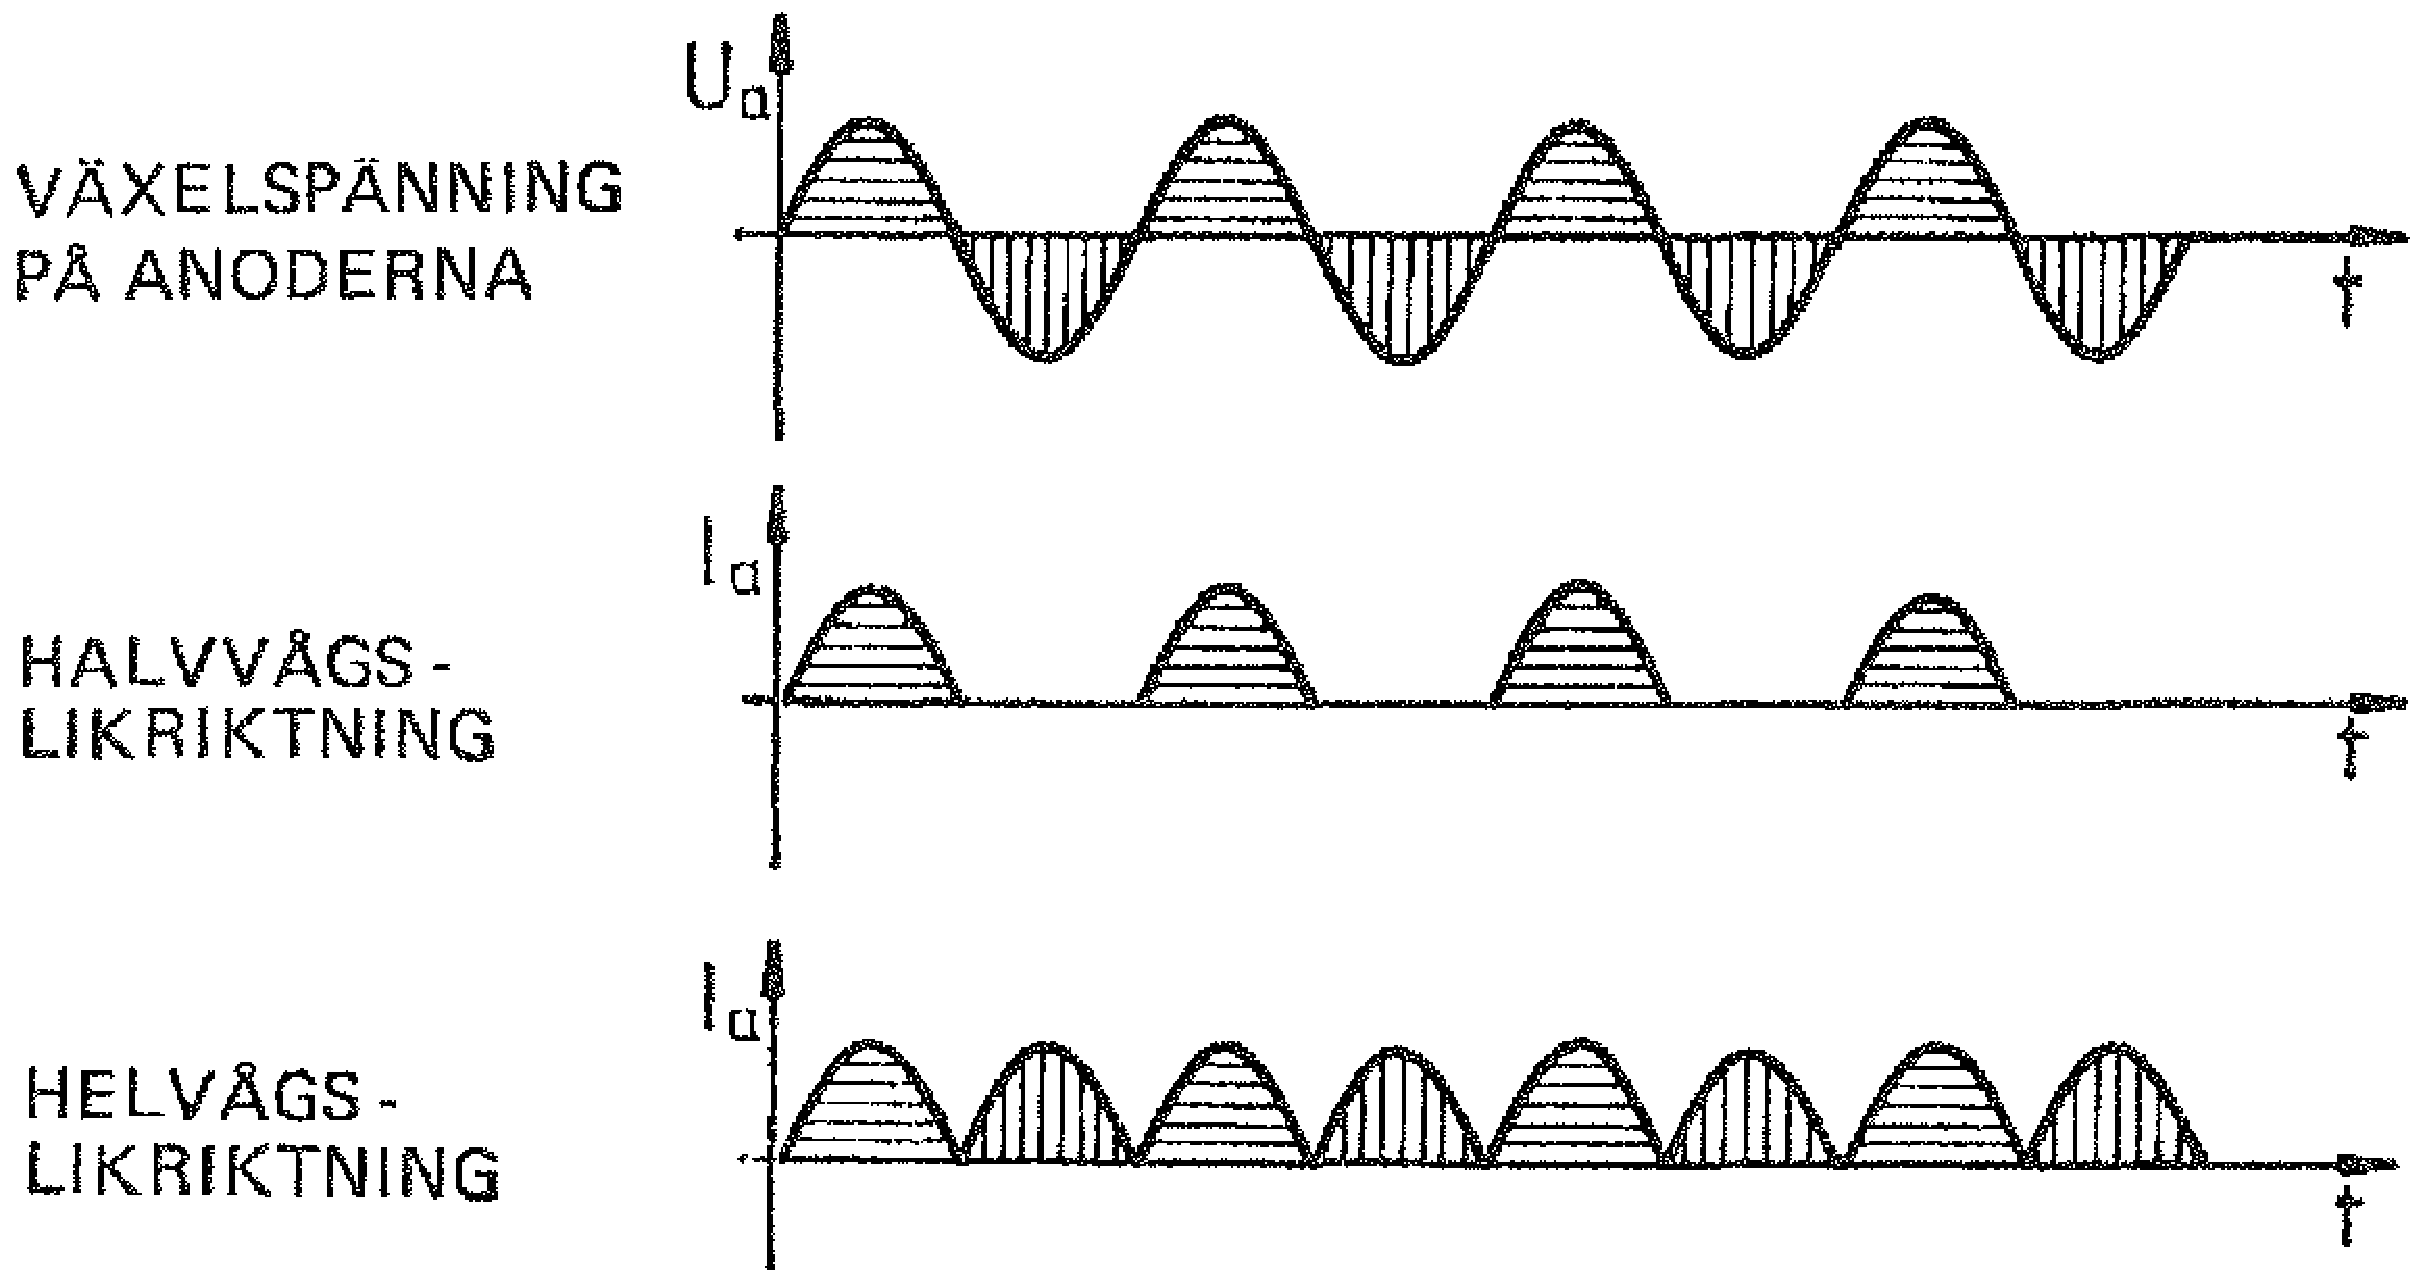
\includegraphics[width=\textwidth]{images/cropped_pdfs/bild_2_2-29.pdf}
\caption{Likriktande funktion}
\label{fig:BildII2-29}
\end{figure}

Bild \ref{fig:BildII2-29}

\subsection{Vakuumtrioden (treelektrodröret)}
\index{vakuumtrioden}
\index{trioden}
\index{elektronrör!triod}

\begin{figure*}[h]
\begin{center}
  %%\begin{wrapfigure}[9]{R}{0.5\textwidth}
  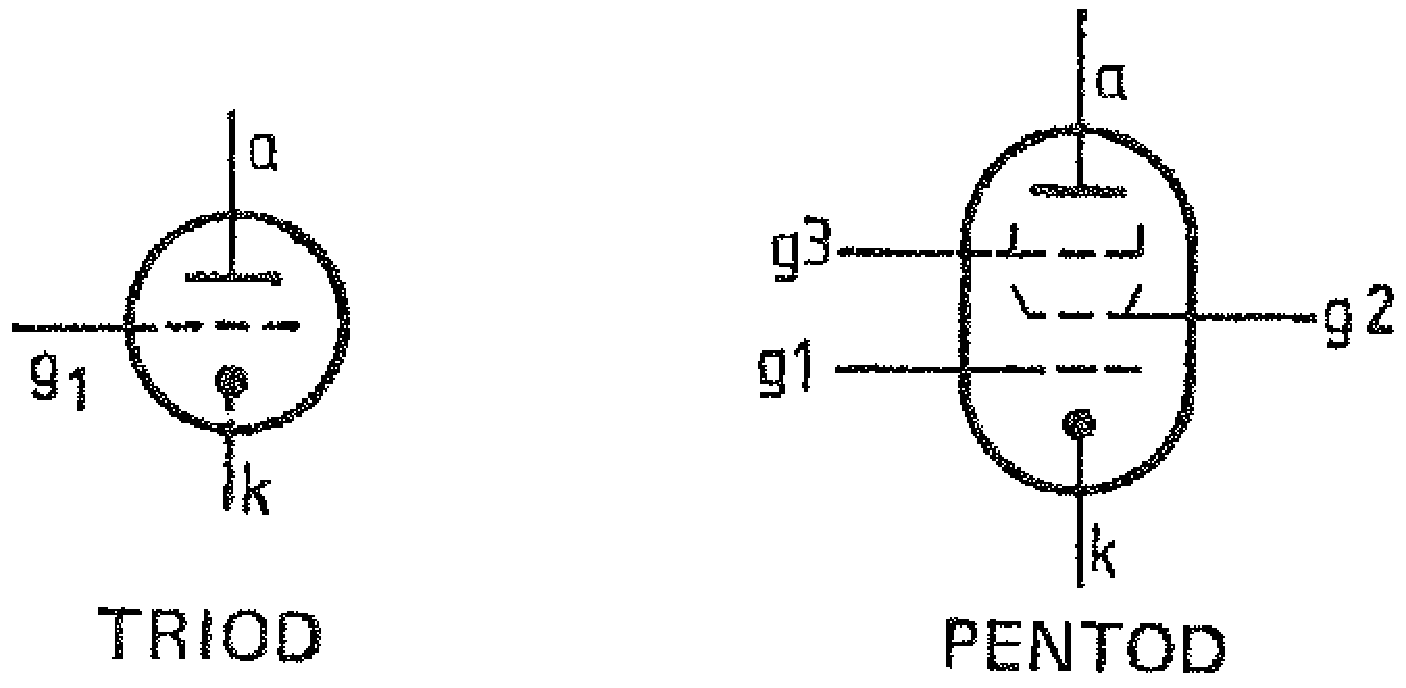
\includegraphics[width=0.5\textwidth]{images/cropped_pdfs/bild_2_2-30.pdf}
  \caption{Symboler för triod och pentod}
  \label{fig:BildII2-30}
  %%\end{wrapfigure}
\end{center}
\end{figure*}

Bild \ref{fig:BildII2-30}

Trioden innehåller tre elektroder
\begin{tabular}{ll}
a & anod \\
\(g_1\) & styrgaller \\
k & katod, med f f = glödtråd \\
  & (filament) \\
\end{tabular}

\subsubsection{Triodens funktion}

Bild \ref{fig:BildII2-31}

En triod fungerar som en diod, när styrgallret ges samma potential som katoden.
Valet av förspänning avgör triodens arbetssätt. styrgallret kan ges positiv,
neutral eller negativ potential (förspänning) i förhållande till katoden. Med
styrgallret positivt ökar anodströmmen. Med gallret negativt minskar den.

Trioden har en \emph{förstärkande} funktion eftersom anodströmmen kan styras med
styrgallret. En liten ändring av gallerspänningen medför stor ändring av
anodströmmen. Vid positiv förspänning flyter det gallerström, som inte får bli
för hög. Vanligen väljs en negativ förspänning.

\begin{figure}[h]
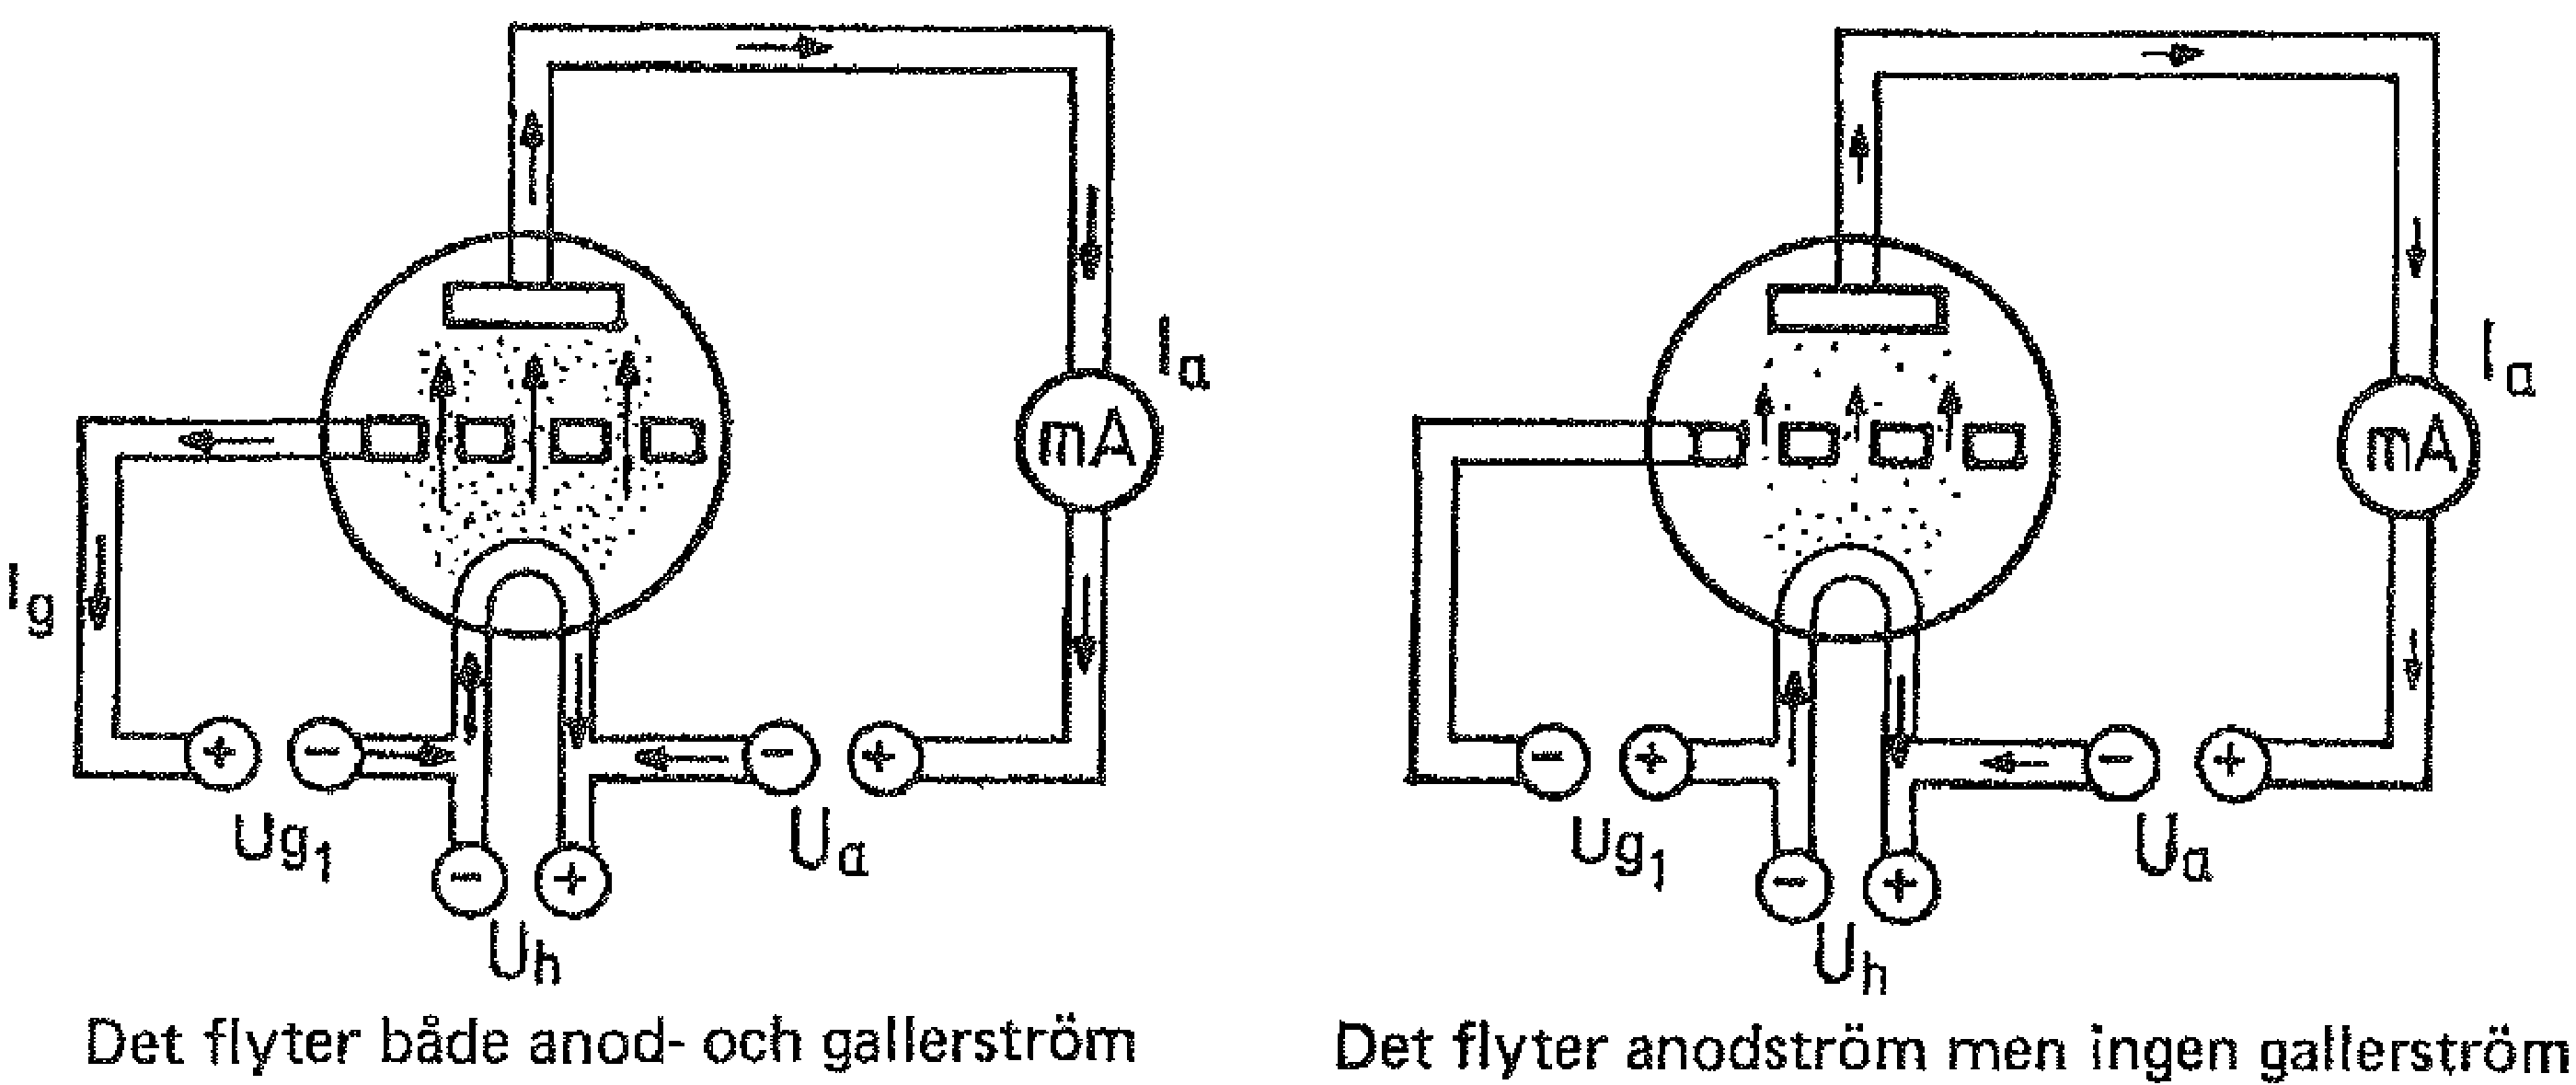
\includegraphics[width=\textwidth]{images/cropped_pdfs/bild_2_2-31.pdf}
\caption{Elektronstömmen i en triod}
\label{fig:BildII2-31}
\end{figure}

\subsubsection{Triodens strömkretsar och strömkällor}

\begin{tabular}{lll}
Glödströmskrets      & Anodkrets        &  Gallerkrets \\
Glödbatteri          & Anodbatteri      &  Gallerbatteri \\
Glödspänning \(U_f\) & Anodsp. \(U_a\)  &  Gallersp. \(U_{g1}\) \\
Glödström \(I_f\)    & Anodstr. \(I_a\) &  Gallerstr. \(I_{g1}\) \\
\end{tabular}

Vanligen används nätdrivna strömkällor i stället för batterier.

Valet av gallerförspänning är avgörande för triodens arbetssätt.

\subsection{Pentoden (femelektrodröret)}
\index{pentod}
\index{elektronrör!pentod}

Pentaden innehåller fem elektroder.

\begin{tabular}{ll}
  a       & anod \\
  \(g_3\) & bromsgaller \\
  \(g_2\) & skärmgaller \\
  \(g_1\) & styrgaller \\
  k      & katod, med f f = glödtråd (filament) \\
\end{tabular}

Bromsgallret förbinds med katoden. Skärmgallret ges en potential som är något
lägre än anodspänningen. Broms- och skärmgallren förhindrar elektronerna att
studsa tillbaka till styrgallret efter anslaget mot anoden.


\subsection{Tetroden (fyraelektrodröret)}
\index{tetrod}
\index{elektronrör!tetrod}

Denna rörtyp innehåller fyra elektroder. Uppbyggnaden är densamma som pentodens,
men bromsgallret saknas.

\subsection{Karaktäristika för elektronrör}

\begin{figure}
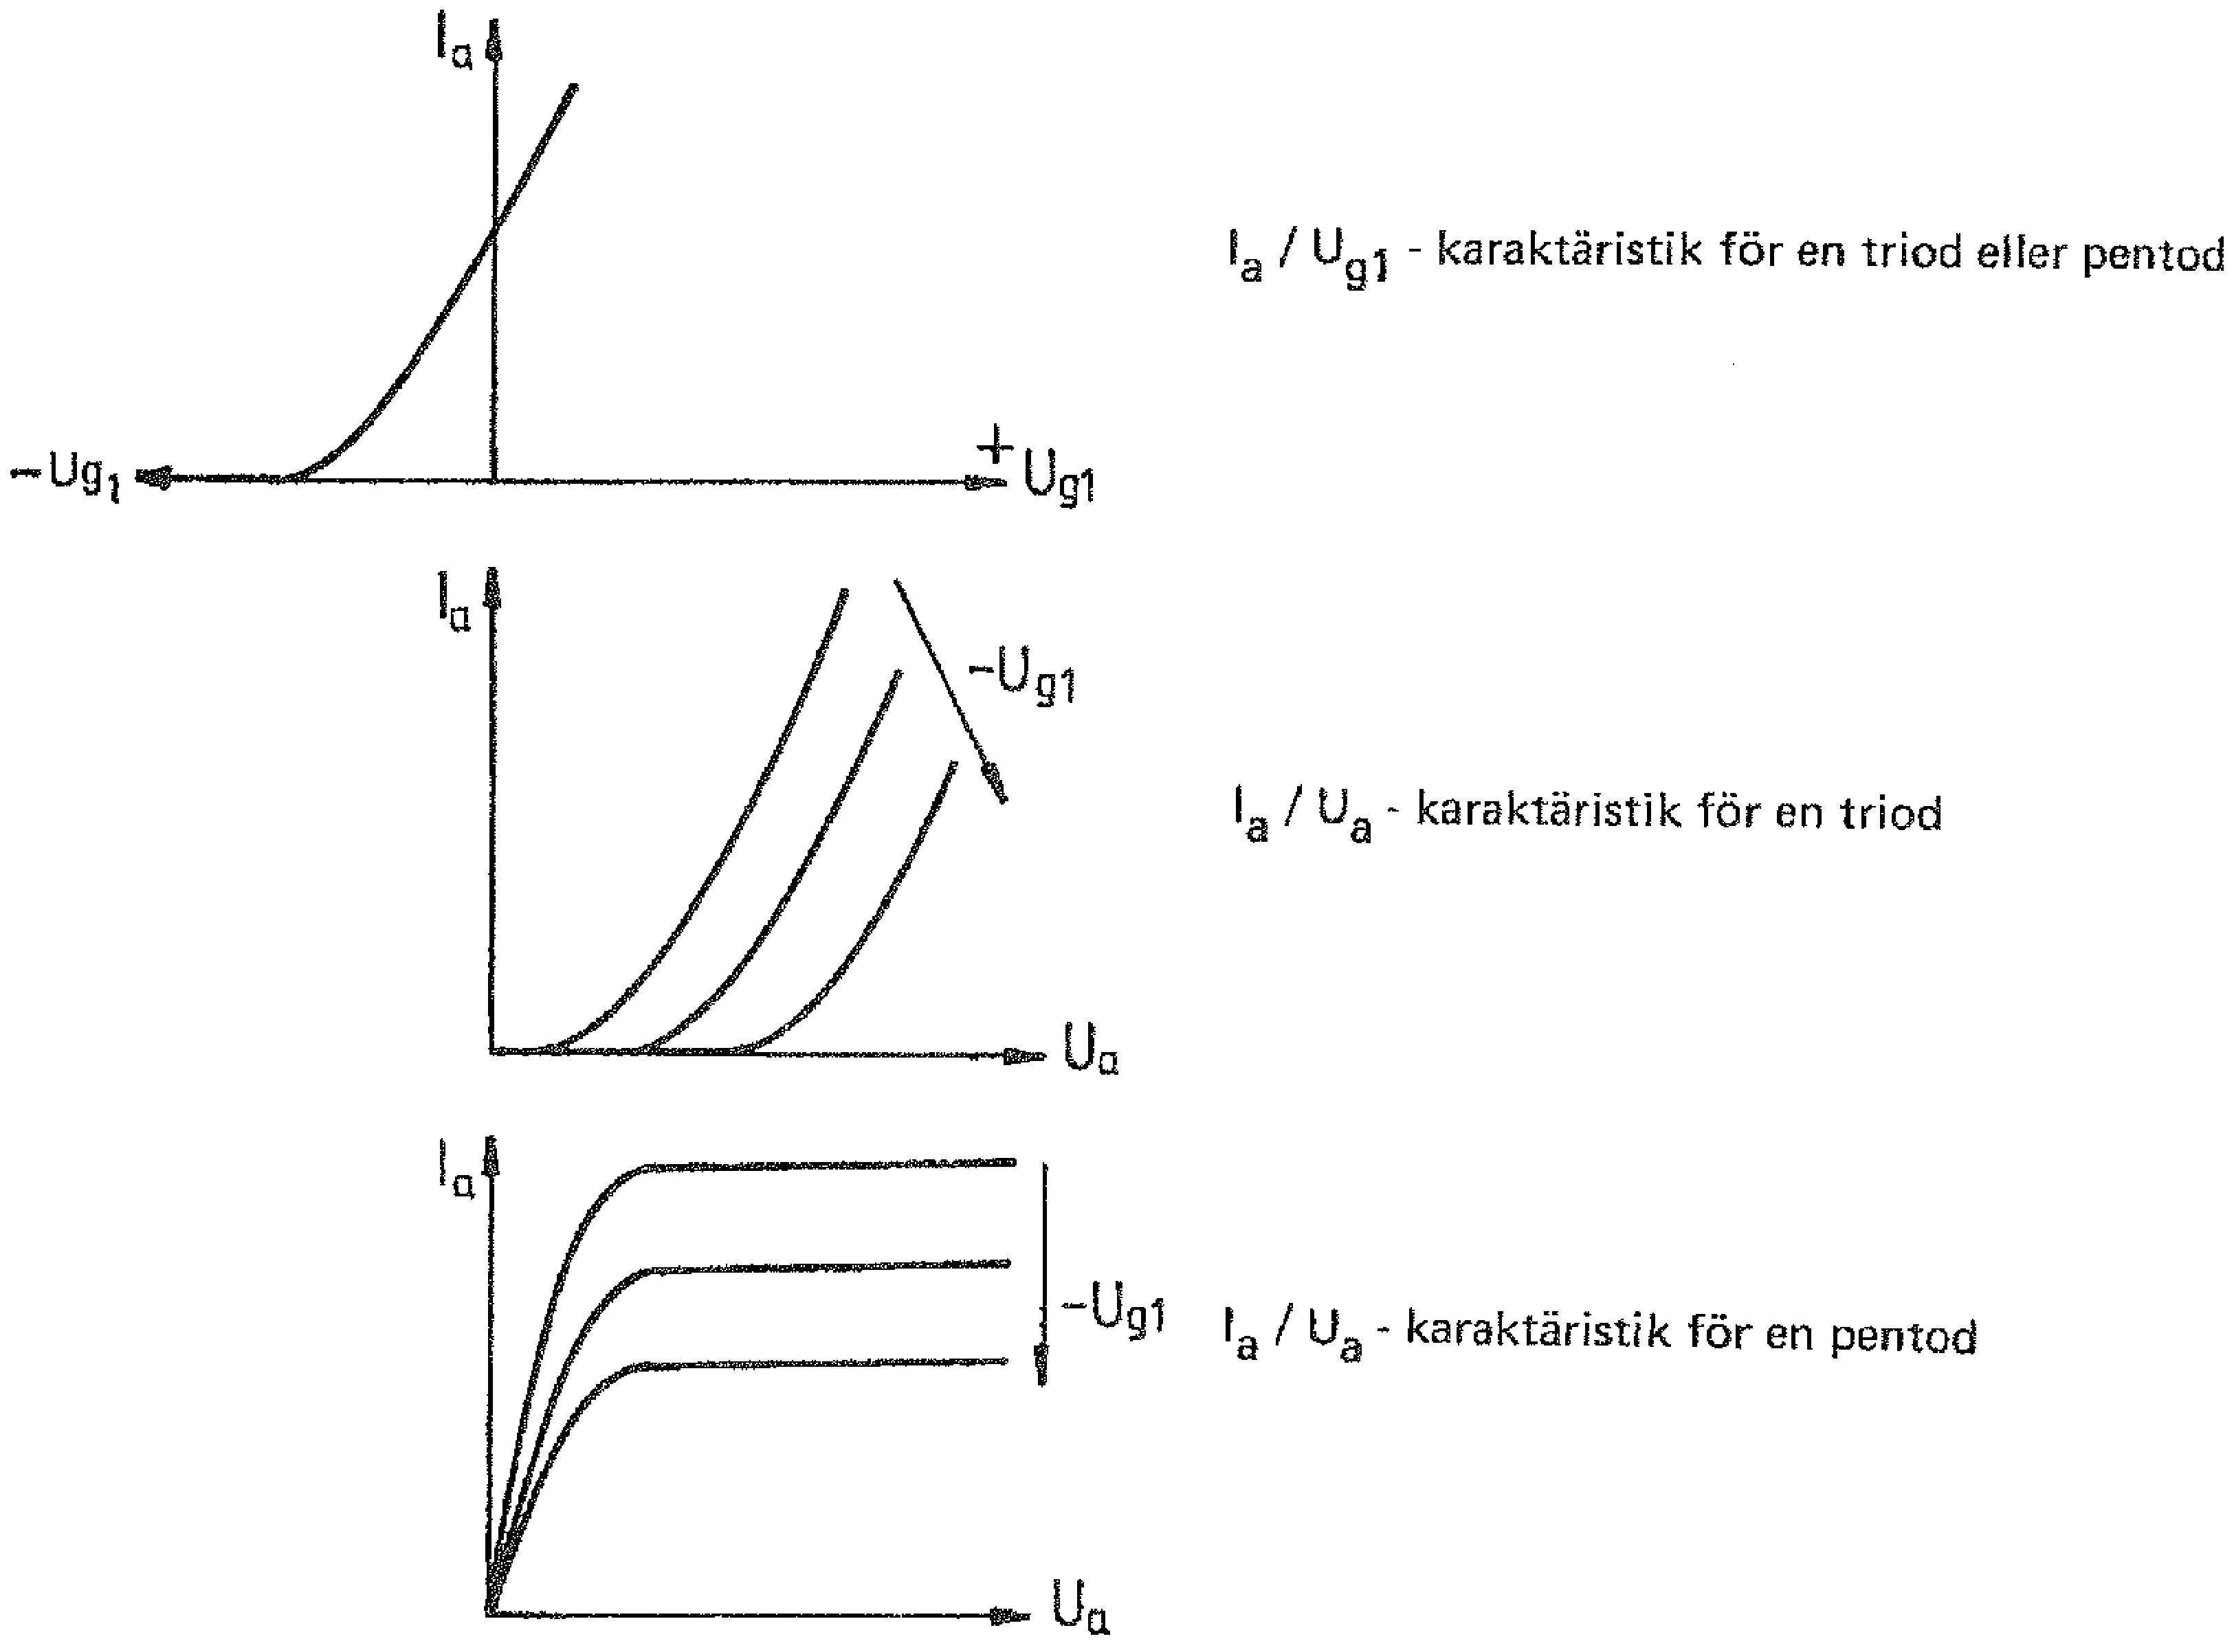
\includegraphics[width=\textwidth]{images/cropped_pdfs/bild_2_2-32.pdf}
\caption{Karaktäristika för elektronrör}
\label{fig:BildII2-32}
\end{figure}

Bild \ref{fig:BildII2-32}

\(I_a/U_{gt}\)-diagram för en triod eller pentod, vid \(U_a\) = konstant

\begin{wrapfigure}[20]{R}{0.5\textwidth}
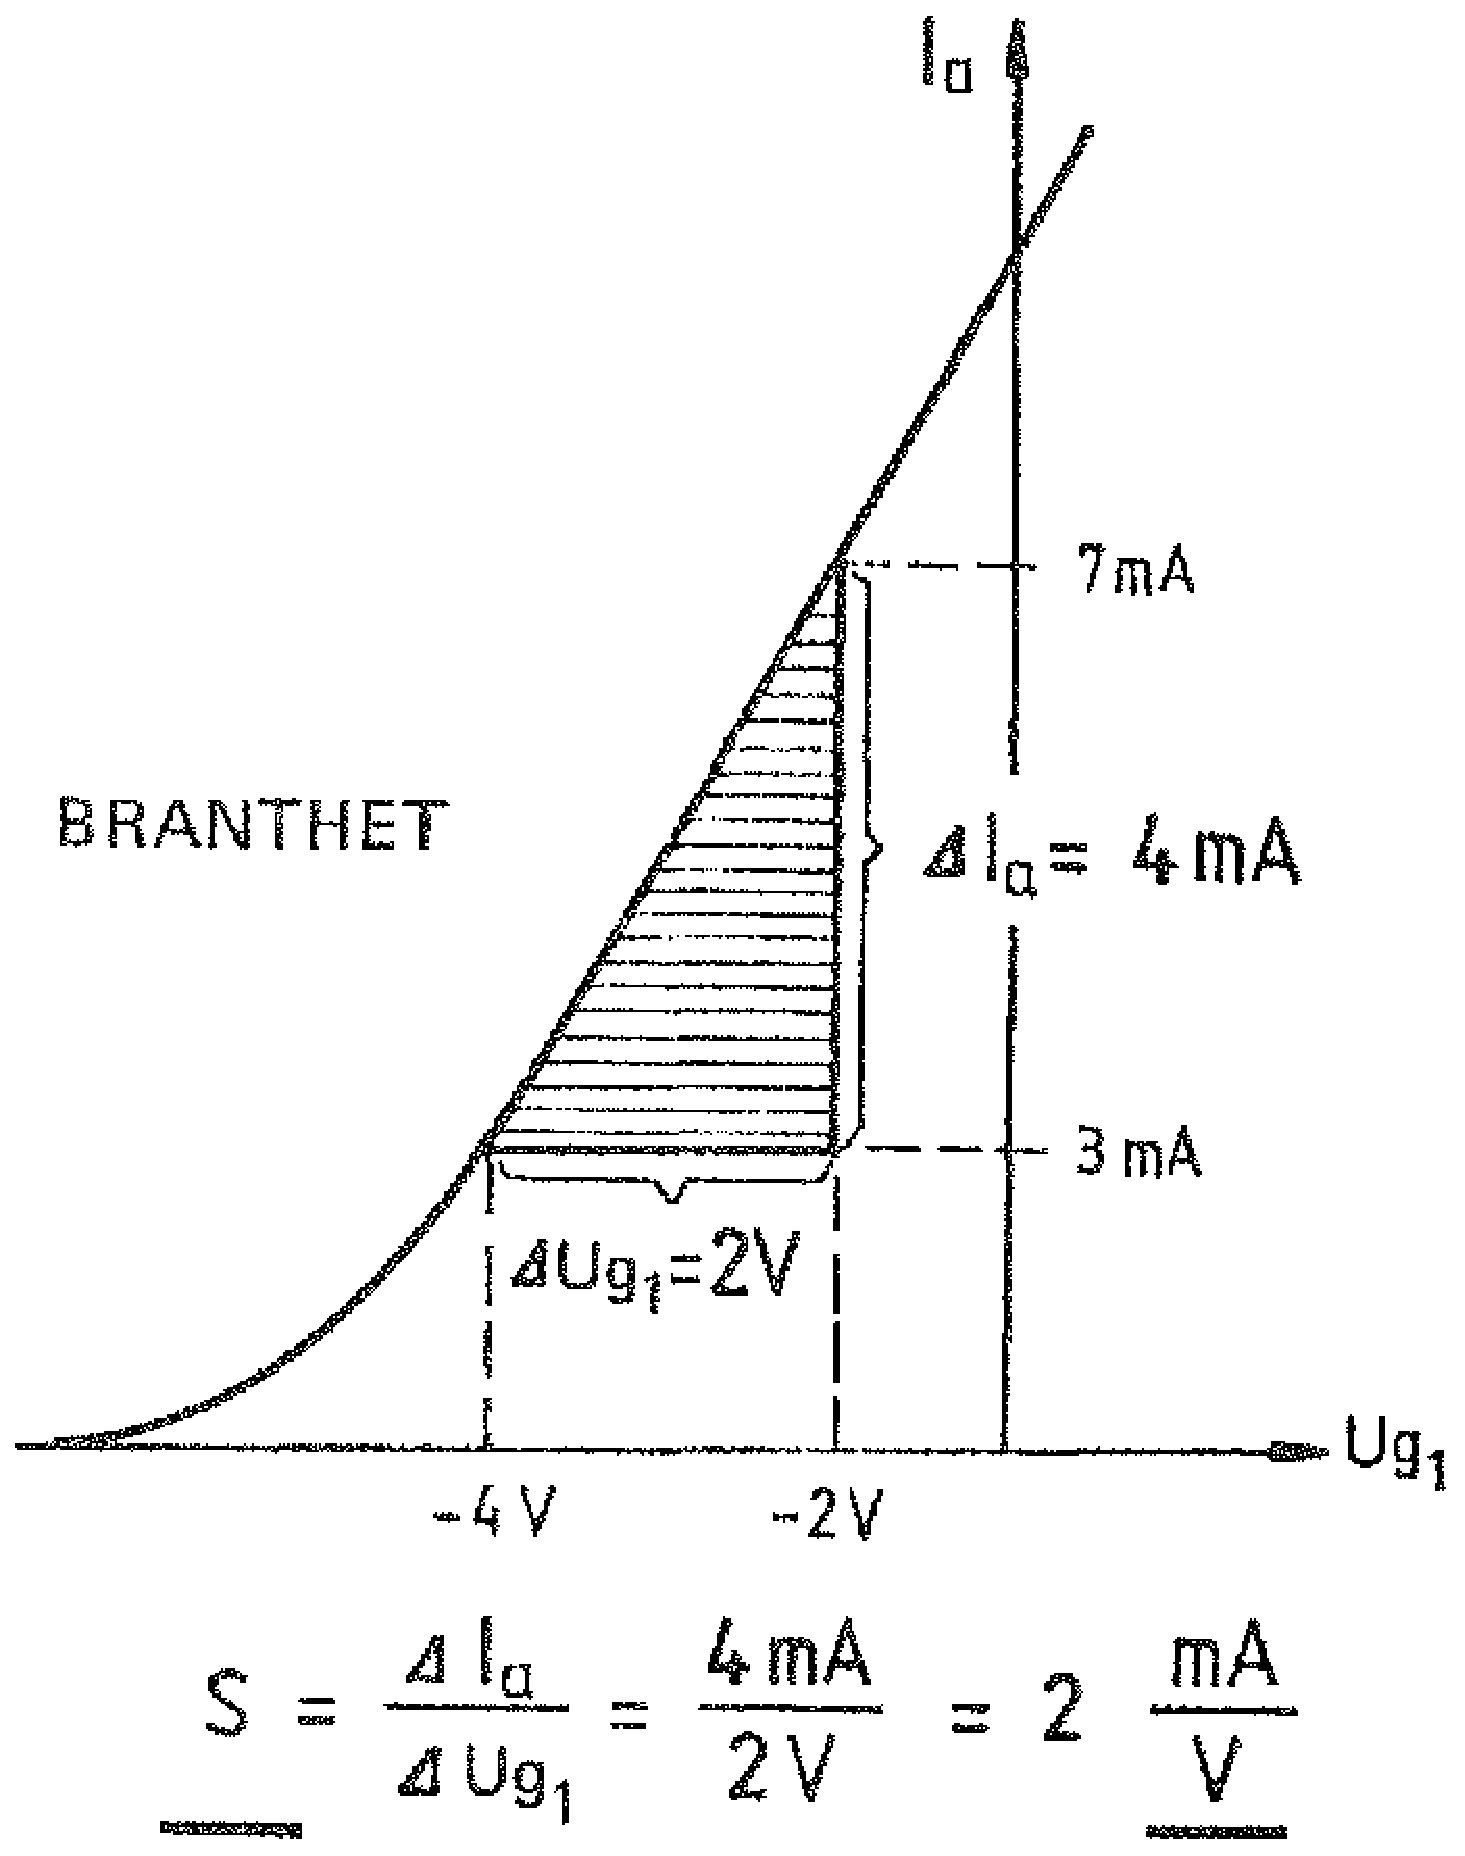
\includegraphics[width=0.5\textwidth]{images/cropped_pdfs/bild_2_2-33.pdf}
\caption{Branthet}
\label{fig:BildII2-33}
\end{wrapfigure}

\(I_a/U_a\)-diagram för en triod, vid \(U_{g1}\) = konstant

\(I_a/U_a\)-diagram för en pentod, vid \(U_{g1}\) = konstant

Tre kurvor visas i \(I_a/U_a\)-diagrammen, med olika värden på
\(U_{g1}\) = konstant (\(U_{g1}\) är s.k. parameter).

\subsection{Branthet $S$ och inre resistans $R_i$}

Bild \ref{fig:BildII2-33}

Om man (vid konstant anodspänning) ändrar gallerförspänningen med värdet
\(∆U_{g1}\) så ändrar sig anodströmmen med värdet \(∆I_a\).

Branthet \(S = \dfrac{∆I_a}{∆U_{g1}}\)

\(S\ [mA/V]\) \(∆I_a\ [mA]\) \(U_{g1}\ [V]\)

Bild \ref{fig:BildII2-34}

Om man (vid konstant gallerförspänning) ändrar anodspänningen med
\(∆U_a\) så ändras anodströmmen med värdet \(∆I_a\).

Inre resistans \(R_i = \dfrac{∆U_a}{∆I_a}\)

\(R_i\ [k \omega]\)  \(∆U_a\ [V]\)  \(∆I_a\ [mA]\)

\begin{figure}[h]
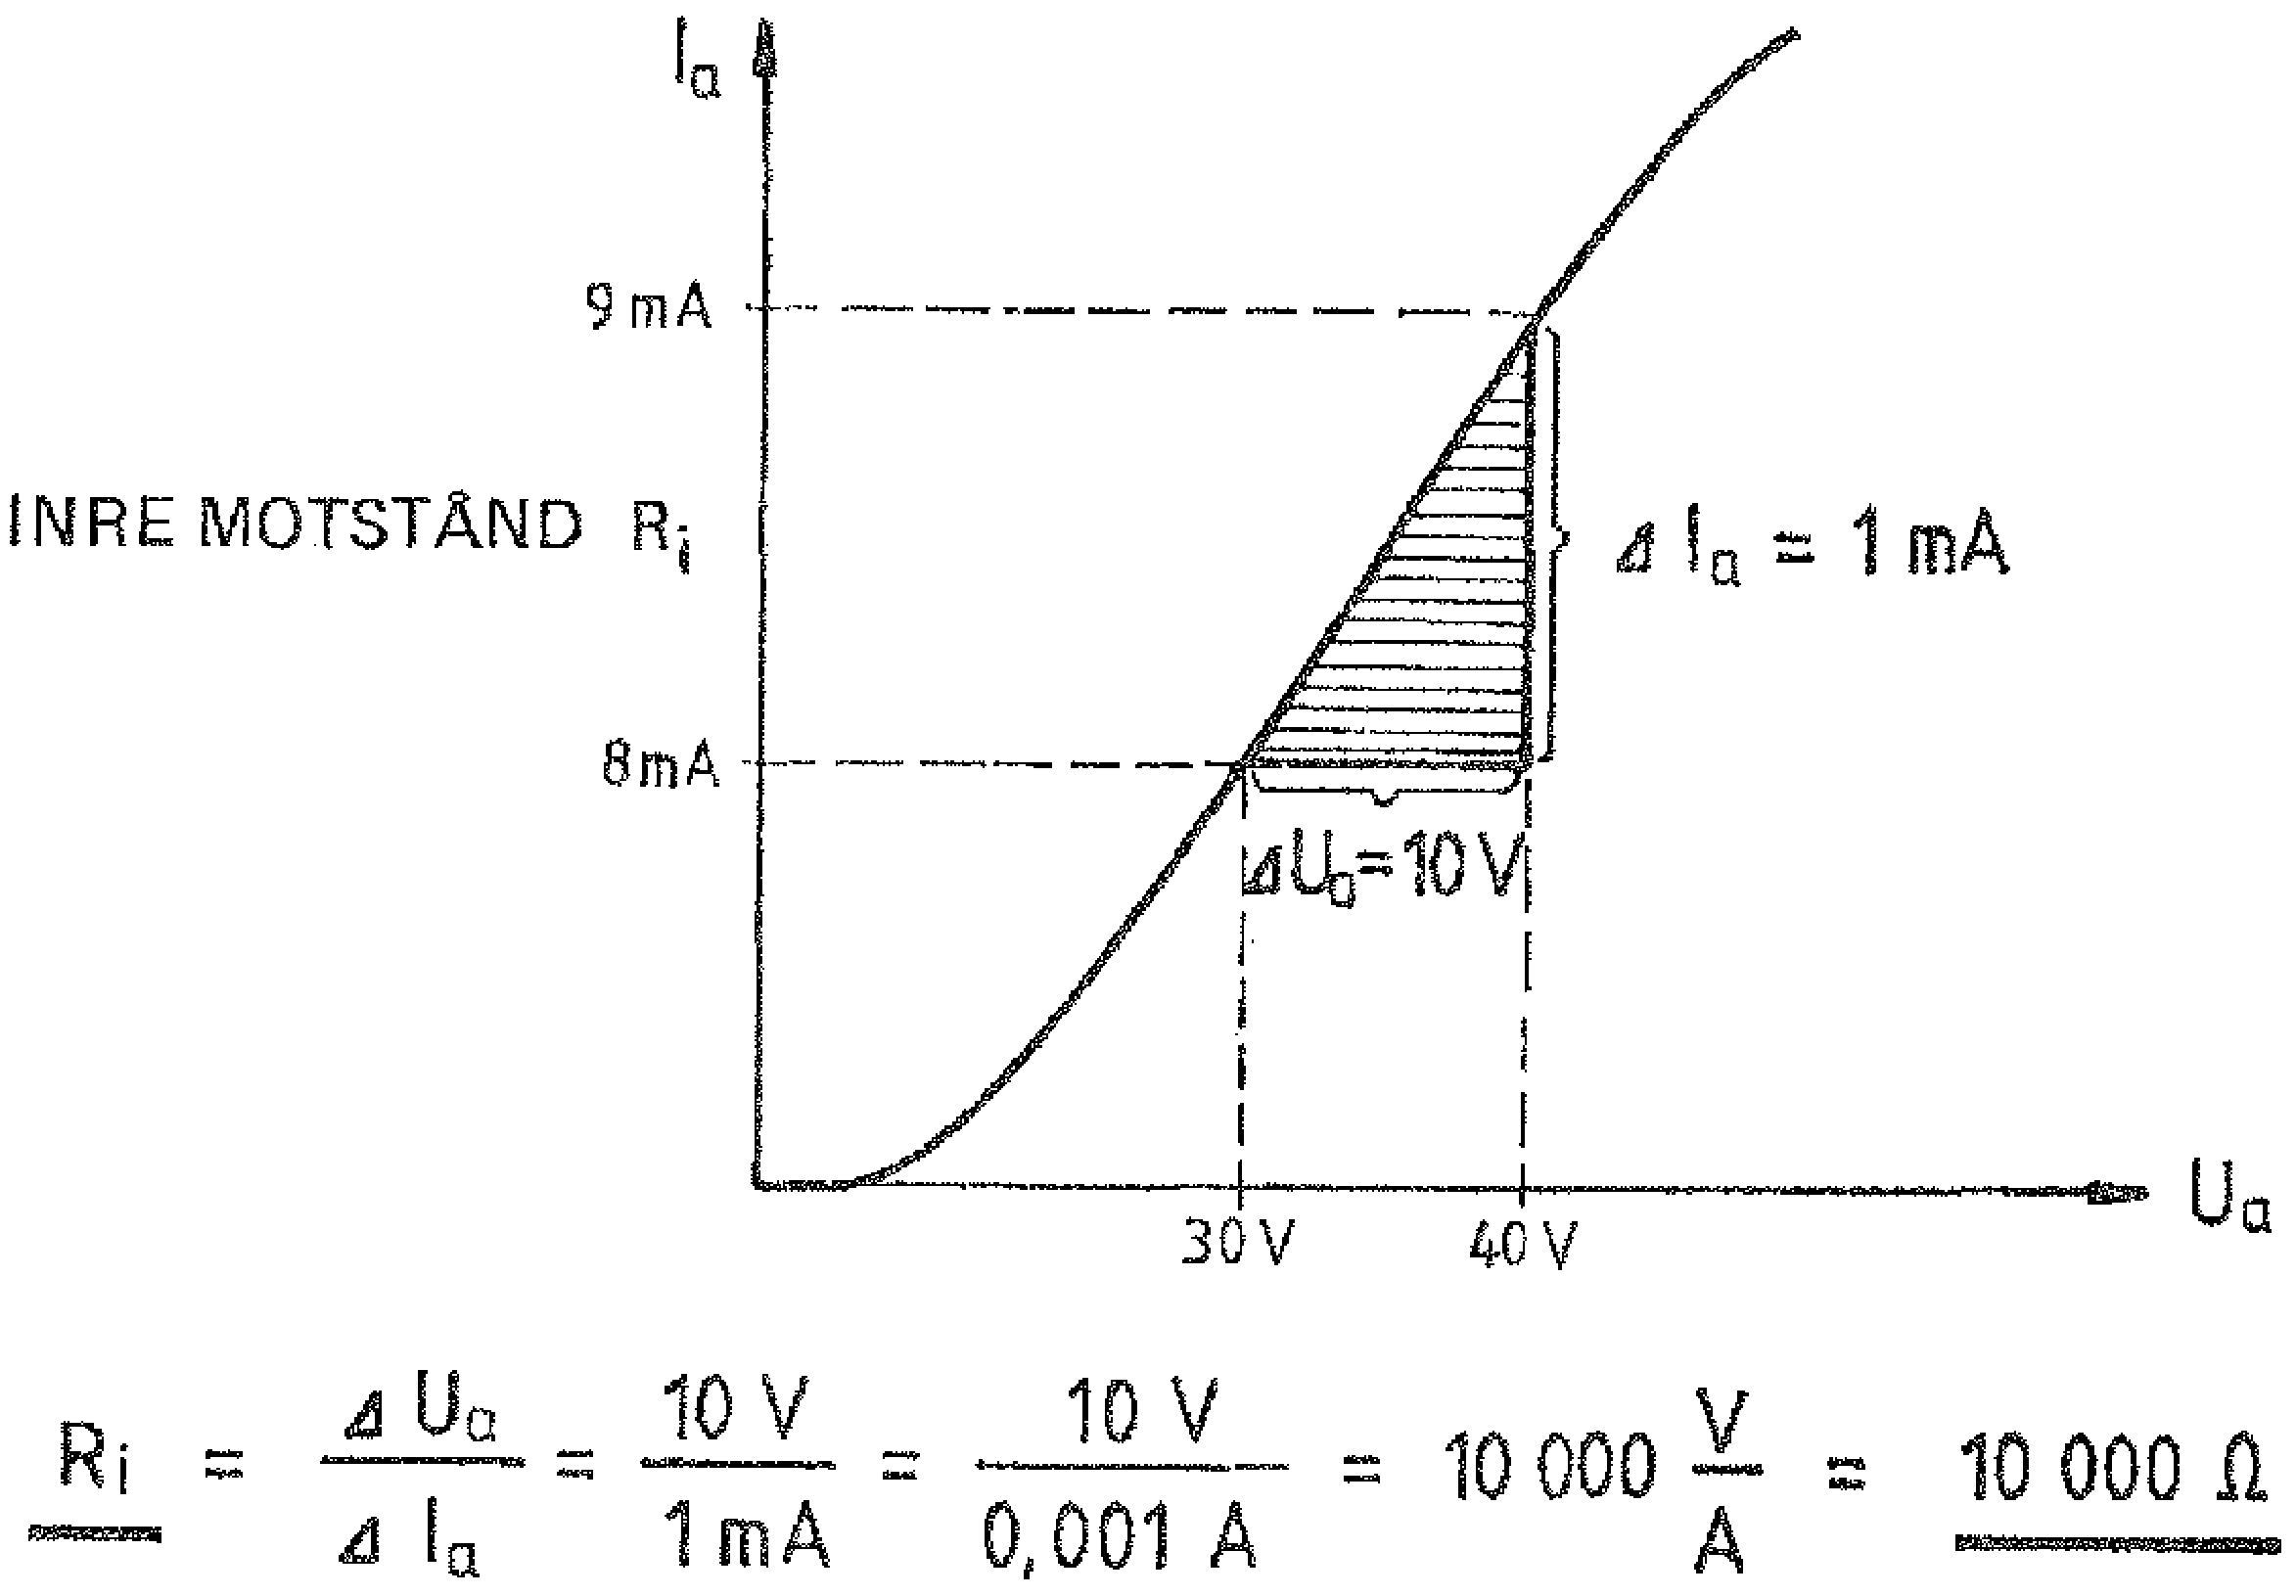
\includegraphics[width=\textwidth]{images/cropped_pdfs/bild_2_2-34.pdf}
\caption{Inre resistans}
\label{fig:BildII2-34}
\end{figure}

Om man vill ändra anodströmmen med ett värde \(∆I_a\), så ges det två
möjligheter:
\begin{itemize}
\item Ändra gallerförspänningen med värdet \(∆U_{g1}\)
\item Ändra anodspänningen med värdet \(∆U_a\).
  Med ändring av gallerförspänningen med värdet \(U_{g1}\) kan man åstadkomma
  samma anodströmsändring \(∆I_a\) som med en ändring av anodspänningen med
  värdet \(∆U_a\).
\end{itemize}

\subsection{Barkhausens elektronrörsformler}
\index{Barkhausen elektronrörsformler}
\index{elektronrör!Barkhausen formler}

\emph{Förstärkningsfaktorn \(\mu \)}

Följande samband gäller mellan de s.k. rörkonstanterna

\(\mu = S \cdot R_i\)

Exempel:

Beräkna \(\mu\)  om \(S = 2\ mA/V\) \(R = 10\ kΩ\) \(\mu = ?\)

Svar: \(\mu = 20\) (\(\mu\)  är dimensionslös)

\subsection{Transistorer jämfört med elektronrör}

\emph{Transistorer}

Fördelar:
\begin{itemize}
\item Lågt pris
\item Små dimensioner
\item Lång livslängd
\item Enkel strömförsörjning (glödström behövs inte)
\item Låg driftspänning (6 V, 12 V \ldots ).
\end{itemize}

Nackdelar:
\begin{itemize}
\item Känslighet för överbelastning och höga temperaturer.
\end{itemize}

\emph{Elektronrör}

Fördelar:
\begin{itemize}
\item Tålighet mot överbelastning
\end{itemize}

Nackdelar:
\begin{itemize}
\item Behöver hög anodspänning
\item Behöver glödström
\item Utrymmeskrävande
\end{itemize}

Ett användningsområde, där elektronrör ännu är vanliga, är i större
sändarslutsteg.

Transistorer ersätter numera nästan helt elektronrören, men man bör ändå känna
elektronrörens egenskaper och arbetssätt.
